\chapter{Introduction}
\label{chap:introduction}

\section{Self-driving solutions}
Nowadays, self-driving cars gain more and more attention, both their technology and their effect on people's daily routines and their lives overall. Several articles are published every year about how these cars will change the way people commute to work, visit their friends or go on a family vacation. These articles often point out the decrease of the number of accidents, an optimized load of traffic and thus a reduced fuel consumption as the major advantages of this technology-to-come.

The release date of these cars, however, is still a matter of question. In 2015, Mark Fields, president and CEO of Ford at the time estimated their first fully autonomous car in 2020. 2 years later, at CES 2017 Nvidia announced that with the partnership of Audi they would develop a self-driving vehicle - also, in market by 2020. Both of these statements are considered too ambitious guesses today, as there is a high probability that we need to wait for at least another decade for reliable fully autonomous vehicles to hit the roads. Claiming that there are no viable signs of these cars in traffic would be a false statement, as there are several companies who have been testing there vehicles on public roads for the last years, but these prototypes are very far from reliable products yet. The company that seems to be ahead of the competition in this race is Tesla. Their self-drving software is already in their products, but it still needs millions of hours of testing and the responsibility is still the driver's if an accident happens.

But why is this delay of release dates? One possible answer is that manufacturers have the tendency to exaggerate when asked about new products, and thus the users' need and the other competitors development speed urged them to make such estimations they could not keep up with. Another theory is that the companies at that time didn't acknowledge how many hours and kilometers of testing is needed to finalize a self-driving product.

However, the spreading of autonomous vehicles is blocked by several legislational and technological obstacles. As this thesis describes an engineering problem an its solution, I will reflect on the technological blockers that both car manufacturers and other self-driving software developer companies need to face. Just to list some of these problems, we can name reliable object detecion, error insensitive, robust decision-making, fast, well-tuned physical control, and to meet the safety and quality requirements set by the market, determinant scheduling and redundancy throughout the whole software are also essential.

Almost all L5 level self-driving applications can be divided into the same sub-tasks, which are perception, environment building, trajectory planning and control.

Perception (or sensor layer) consists of managing a sensor setup that is able to provide the car with the necessary information about its environment and its own state to create a realistic model of the world. One of the hardest question in this area of engineering is how many and what type of sensors to use. It is especially important for automotive manufacturers, for reducing the price of a sensor set on a car makes manufacturing more profitable. Typical sensor setups include 4 front and 4 rear radars for short-range measurements (typically parking purposes), long-range radars facing forward and backward, IMUs\footnote{Inertial measurement units are electronic devices that measure and report a body's specific force, angular rate, and sometimes the orientation of the body, using a combination of accelerometers, gyroscopes, and sometimes magnetometers. (source: \href{https://en.wikipedia.org/wiki/Inertial_measurement_unit}{Wikipedia})} and GPS receivers. Camera-based solutions (like the one Budapest-based AImotive is developing) may also need front- and rear-facing mono- and/or stereo-cameras and fish-eye cameras on the side. Other approaches use LIDARs placed on top of the car (e.g. Uber and Waymo). The price of these laser scanners are sometimes higher than the car they are applied on. While trying to keep them as minimal as possible, manufacturers must create sensor setups that will be fit for the needs of future fully autonomous programs, which may not be estimated currently today. After the setup has been decided on, the perception layer is still in need of an enermous amount of engineering, as it is responsible for handling these sensors - calibrating them, reading and filtering their values, and forwarding them to the upper-level components of the chain.

Using the filtered, but still raw output of the sensor handling components, these softwares need to make a realistic and fine-grained map of the world surrounding the vehicle. This environment-building sub-task requires various different, preferably independent input sensors, and it implements the fusion of these data. While its inputs are raw camera images, 2D or 3D LIDAR scans and radar measurements, its output is a 2D or 3D (depending on the application) map of the world, possibly published in a standard format for further evaluation. Among many problems this step has to solve are the different measurement frequencies of the sensors (cameras used in seld-driving solutions typically record video at 30 frame/sec, while automotive LIDARs rotate at maximum 20 Hz), the sensor noise that still remains after filtering, and also contradicting measurements coming from different sensors.

The built world model is used by trajectory-planning that calculates an optimal path for the target destination. This path should avoid any obstacles that may cause a collision. This step requires detailed information about the physical dimensions and kinematics of the objects in the map, and also about the driven vehicle's capabilities (such as maximum acceleration or maximum wheel angle) - note, that these values are strictly limited according to automotive standards and safety measurements.

Once the desired trajectory has been calculated, the control module has the task to actually \textit{drive} the car. It controls the actuators, and its aim is to follow the path as strictly as possible. This steps needs a well-detailed picture of the controlled car's characteristics, which can be obtained via in-depth identification.

All important players in the automotive industry are developing some kind of self-driving, using different software architectures defined by the above modules.

\section{The \textit{vr-car} project}
The Department of Automation and Applied Informatics at the Budapest University of Technology and Economics also has a team developing a self-driving solution - however, in a much smaller scale. The department is well-known for organizing or taking part in several robotics and autonomous projects. The \textit{vr-car} project is based on model car of 1:3 scale, which is applied with several computers, sensors and actuators in order to make it fit for testing self-driving algorithms.

\begin{figure}[!ht]
    \centering
    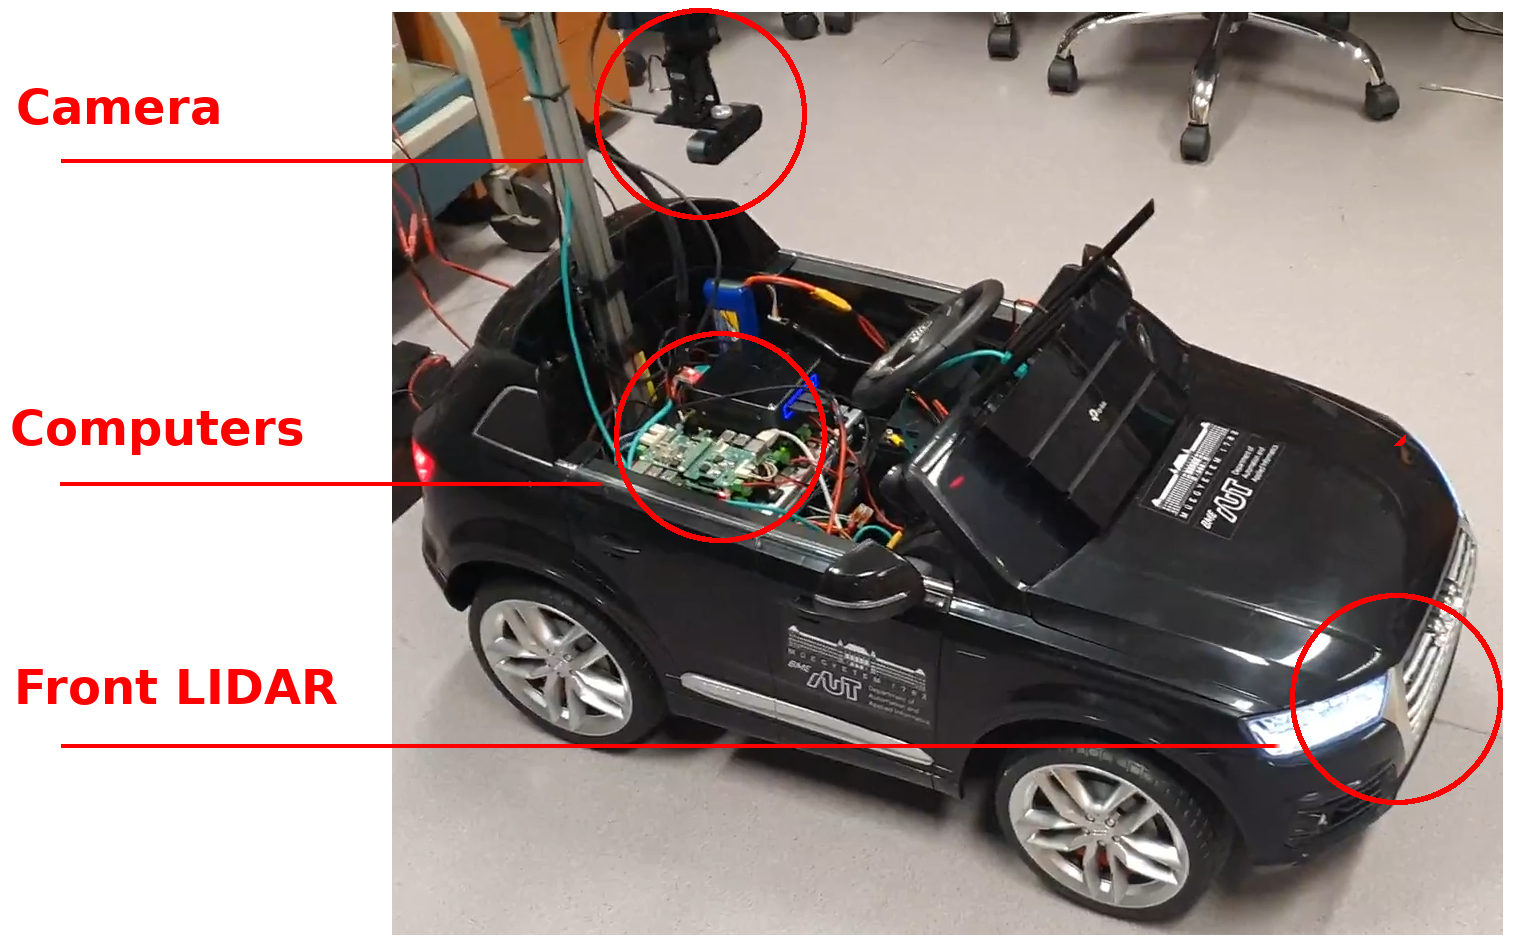
\includegraphics[height=80mm]{figures/raw/car_setup_front.png}
    \caption{The car setup (front side)}
    \label{car_setup_front}
\end{figure}

\begin{figure}[!ht]
    \centering
    \includegraphics[height=100mm]{figures/raw/car_setup_rear.png}
    \caption{The car setup (rear side)}
    \label{car_setup_rear}
\end{figure}
